\chapter{Immersed Boundary Methods}
\label{chpt:IBM}

% ---------------------------------------------------------------------------
% Placeholder for figures that have not been made yet. Replace each
% \IBfigplaceholder{...} with \includegraphics once the figure exists.
% ---------------------------------------------------------------------------
\providecommand{\IBfigplaceholder}[1]{%
  \fbox{\parbox[c][#1][c]{0.85\textwidth}{\centering\sffamily\small
  \textbf{[Figure to be added]}}}}

Immersed boundary methods (IBMs) are built from a numerical framework for
\emph{fluid--structure interaction} (FSI) and specifically designed to model interactions where an object is immersed in a viscous, incompressible fluid. The method was introduced by Peskin to
simulate blood flow around heart valves \parencite{peskin1972} and has
since been used for swimming organisms, cell mechanics, vesicles, flexible
fibers, and many other systems \parencite{peskin2002, mittalIaccarino2005}.
\index{immersed boundary method}

Let's consider an object (a heart valve leaflet, a red blood cell, a wire frame) completely
submerged, or \textit{immersed}, in a fluid domain. If we were to implement the methods of
Chapter~\ref{chpt:FDM} directly, we need a \textit{body-fitted mesh} (or grid) that conforms to the
object so that boundary conditions can be imposed on the immersed object. These meshes are tedious to build for complex geometries and must be rebuilt at every time step if the
object moves or deforms. For a system stepping forward at approximately $10^{-4}$ seconds, this remeshing process is expensive and difficult to implement, especially in three dimensions.

IBMs avoid body-fitted meshes entirely through the use of two grids: one for the fluid field and one for the immersed object. The PDEs that describe the fluid system are solved on the
same uniform Eulerian grid we have used all along, ignoring the object
completely. The object is then described by its own set of curvilinear, Lagrangian points and its
effect on the fluid system is simply imposed onto the fluid domain.

Everything we need to implement a basic IBM
has appeared in earlier chapters: the five-point Laplacian
(Chapter~\ref{chpt:FDM}), block systems with a constraint
(Chapter~\ref{chpt:staggered}), and matrix-free GMRES
(Chapter~\ref{chpt:GMRES}). For those curious, a similar and more in-depth treatment can be found in Peskin's
lecture notes \parencite{peskinNotes}.





\begin{figure}[htbp]
  \centering
  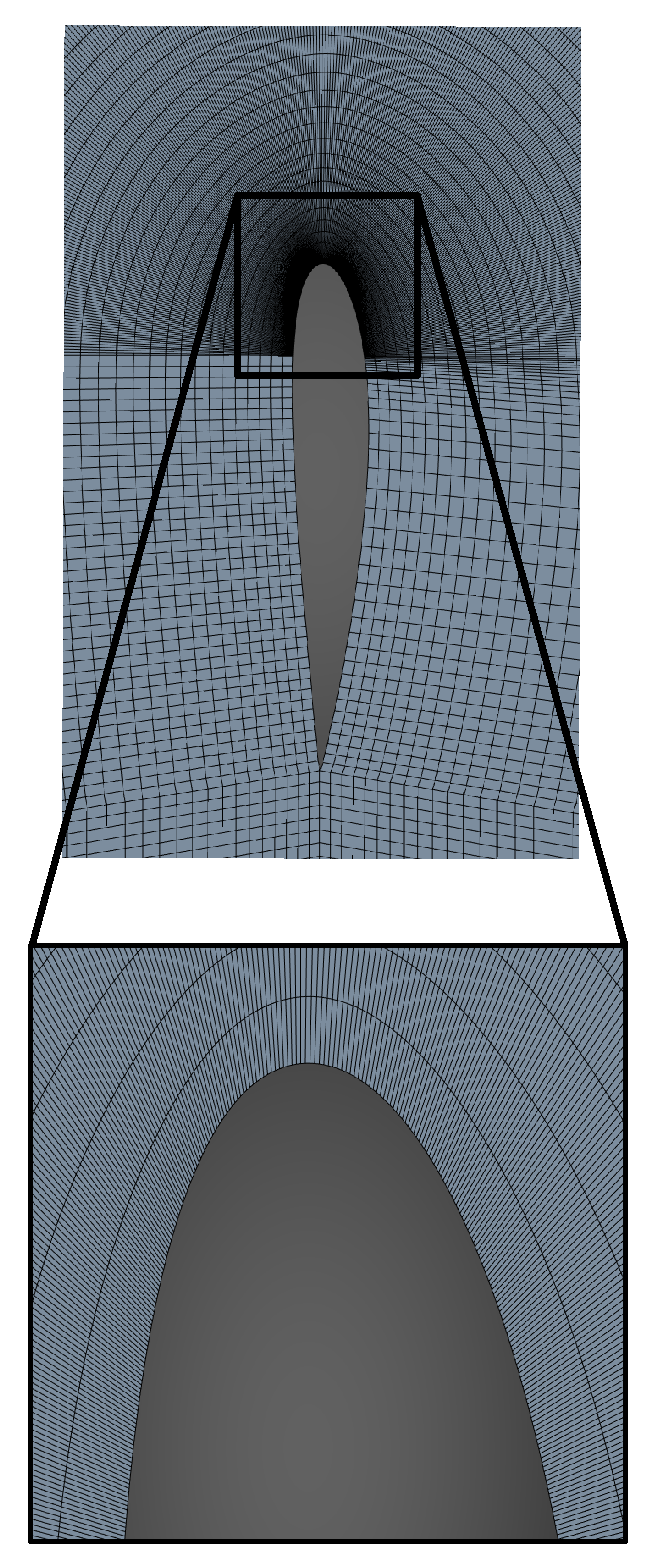
\includegraphics[angle=90, width=\linewidth]{IBM/images/bodyFittedExample.pdf}

  \vspace{1em}

  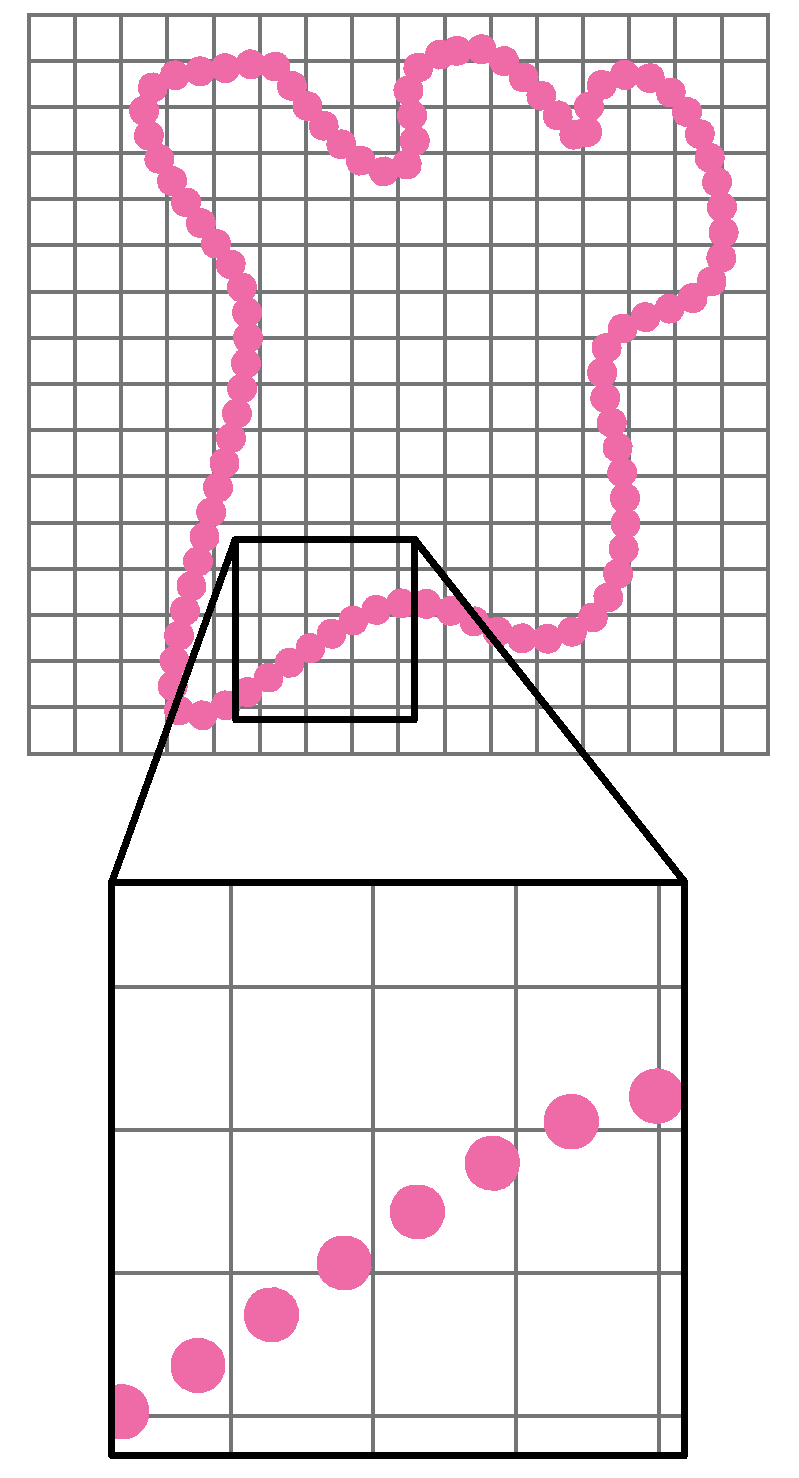
\includegraphics[angle=90, width=\linewidth]{IBM/images/ibExample.pdf}
  \caption{Two ways to discretize a fluid domain containing a closed
  curve on which a boundary condition is imposed. Top: a body-fitted
  (unstructured) mesh whose edges conform to the curve (a NACA 2415
  airfoil, meshed in Ansys Fluent \parencite{ansys}). Bottom: a uniform
  Cartesian grid with the curve drawn on top and represented by its own
  set of points (markers) that do not coincide with grid nodes.}
  \label{fig:IBbodyfitted}
\end{figure}

\begin{remark}
Throughout this chapter, the term \emph{immersed boundary} refers to the
object inside the domain, not to the edge of the computational domain. The
domain edge is handled by ordinary boundary conditions, exactly as in
Section~\ref{sec:2Dbcs}.
\end{remark}




\section{A Model Problem}
\label{sec:IBmodel}
This chapter will work through a model problem to help develop the basic ideas of IBMs.

Let $\Omega = [0,2\pi]\times[0,2\pi]$ define the domain and consider
\begin{equation}
  \nabla^2 u = f \quad \text{in } \Omega, \qquad
  u |_{\partial\Omega} = 0.
  \label{eq:IBpoisson}
\end{equation}
Note this is just the Poisson problem of \eqref{eq:2Dpoisson}. Let $\Gamma$ be the ellipse
\begin{equation}
  \Gamma: \quad X(\theta) = \pi + 1.5\cos\theta, \qquad
  Y(\theta) = \pi + 0.75\sin\theta, \qquad 0 \le \theta < 2\pi.
  \label{eq:IBellipse}
\end{equation}
Let $g(\theta)$ describe the values of $u$ on $\Gamma$, such that
\begin{equation}
  u\big(X(\theta), Y(\theta)\big) = g(\theta), \qquad 0 \le \theta < 2\pi.
  \label{eq:IBring}
\end{equation}

To enforce this condition, we add a force that acts only along the curve
$\Gamma$. We describe it by a force per unit length $\lambda(s)$, where $s$
is arc length along $\Gamma$. \eqref{eq:IBpoisson} can then be rewritten as
\begin{equation}
  \nabla^2 u = f + \int_{\Gamma} \lambda(s)\,
  \delta\big(\mathbf{x} - \mathbf{X}(s)\big)\,ds,
  \label{eq:IBpoissonlambda}
\end{equation}
where $\mathbf{X}(s)$ is the point on $\Gamma$ and
$\delta(\mathbf{x}) = \delta(x)\,\delta(y)$ is the two-dimensional Dirac
delta function. The force density $\lambda$ is a new unknown and
\eqref{eq:IBring} is the equation that determines it.


\subsection{Two Descriptions}
\label{sec:IBdescriptions}

Two different sets of points are used at once, and keeping them separate
is the most important bookkeeping in IB methods.

\begin{definition}
\textbf{Eulerian variables} are functions of a fixed spatial position
$\mathbf{x} \in \Omega$. The solution $u$ and the force $f$ are Eulerian.
They are defined on the same grid we have used in previous chapters.
\end{definition}

\begin{definition}
\textbf{Lagrangian variables} live on the immersed boundary and are
functions of a coordinate along it, here the angle $\theta$. The points of
the curve $\mathbf{X}(\theta)$, the boundary values $g(\theta)$, and the
charges $\lambda$ are Lagrangian.
\end{definition}
\index{Eulerian description}\index{Lagrangian description}

Now we discretize the problem. Let $\Gamma$ be represented by $N_{ib}$ IB points
$\mathbf{X}_k = \big(X(\theta_k), Y(\theta_k)\big)$, with
$\theta_k = k\,\Delta\theta$ with $\Delta\theta = 2\pi/N_{ib}$ for
$k = 0,\dots,N_{ib}-1$. The local spacing between IB points is
$\Delta s_k = |\mathbf{X}'(\theta_k)|\,\Delta\theta$ and, as spacing on an ellipse is not uniform in arc length, the average space is the
perimeter of $\Gamma$ divided by $N_{ib}$. On the IB points, the line
integral in \eqref{eq:IBpoissonlambda} becomes a sum of point charges,
\begin{equation}
  \nabla^2 u = f + \sum_{k=0}^{N_{ib}-1} q_k\,
  \delta(\mathbf{x} - \mathbf{X}_k),
  \qquad q_k \approx \lambda(s_k)\,\Delta s_k,
  \label{eq:IBpoissonq}
\end{equation}
and the condition \eqref{eq:IBring} becomes $u(\mathbf{X}_k) = g_k$ with
$g_k = g(\theta_k)$.
\section{Regularized Delta Functions}
\label{sec:IBdelta}
\index{immersed boundary method!regularized delta function}

A classic delta function cannot be represented on a grid. We will replace it
the Gaussian

\begin{equation}
  \delta_a(x, y) = \frac{1}{2\pi a^2}\,
  \exp\!\left(-\frac{x^2 + y^2}{2a^2}\right)
  = \underbrace{\frac{e^{-x^2/2a^2}}{\sqrt{2\pi}\,a}}_{\delta_a(x)}\;
    \underbrace{\frac{e^{-y^2/2a^2}}{\sqrt{2\pi}\,a}}_{\delta_a(y)},
  \label{eq:IBgauss}
\end{equation}
where the width $a$ is tied to the grid spacing, $a = c\,\Delta x$ for a
constant $c$ of order one. In this chapter we take $a = 1.2\,\Delta x$. As
$\Delta x \to 0$, $\delta_a$ becomes narrower and taller and approaches the
true delta function. Using a Gaussian in this way is the idea behind the
\emph{force coupling method} \parencite{maxeyPatel2001}, and the Gaussian delta function
is the only part of this chapter that differs from Peskin's version of the
method.

On the grid, integrals become sums. The property we need most is that the
discrete version of $\int \delta_a(x - X)\,dx = 1$ holds no matter where
$X$ sits relative to the grid:
\begin{equation}
  \sum_i \delta_a(x_i - X)\,\Delta x \approx 1 .
  \label{eq:IBunity}
\end{equation}

\begin{remark}
The Gaussian is never exactly zero, so in principle every IB point
touches every grid point. To make this more realistic and cost-effective, we would want to define a \textit{support} for each delta function so it only impacts subsets of the domain.
\end{remark}

\subsection{Peskin's Four-Point Kernel}

\index{immersed boundary method!four-point kernel}
\index{compact support}
Peskin's original method uses a kernel with \emph{compact support}. His
four-point kernel \parencite{peskin2002} is written in terms of the
distance to a grid point measured in grid cells, $r = x/\Delta x$, as
$\phi(r) = \Delta x\,\delta_h(x)$ with
\begin{equation}
  \phi(r) =
  \begin{cases}
    \dfrac{3 - 2|r| + \sqrt{1 + 4|r| - 4r^2}}{8}, & 0 \leq |r| \leq 1,\\[3mm]
    \dfrac{5 - 2|r| - \sqrt{-7 + 12|r| - 4r^2}}{8}, & 1 \leq |r| \leq 2,\\[3mm]
    0, & 2 \leq |r|,
  \end{cases}
  \label{eq:IBphi4}
\end{equation}
and $\delta_h(x,y) = \delta_h(x)\,\delta_h(y)$ in two dimensions. Rather
than being chosen for its shape, \eqref{eq:IBphi4} is the unique function
that satisfies the following conditions, where the sums run over all
integers $j$ and must hold for every real $r$:
\begin{enumerate}[label=(\roman*)]
  \item $\phi(r)$ is continuous;
  \item $\phi(r) = 0$ for $|r| \geq 2$;
  \item $\displaystyle\sum_{j\ \mathrm{even}} \phi(r - j)
        = \sum_{j\ \mathrm{odd}} \phi(r - j) = \frac{1}{2}$;
  \item $\displaystyle\sum_{j} (r - j)\,\phi(r - j) = 0$;
  \item $\displaystyle\sum_{j} \phi(r - j)^2 = \frac{3}{8}$.
\end{enumerate}
Each condition has a purpose. Continuity (i) keeps the interaction smooth
as an IB point slides across the grid. Compact support (ii) means each IB
point touches exactly a $4 \times 4$ block of grid points, which makes
spreading and interpolation cheap. Adding the two sums in (iii) gives
\eqref{eq:IBunity} exactly, so the total charge is conserved when it is
spread; requiring the even and odd sums separately also prevents a
checkerboard pattern that centered differences cannot see. Condition (iv)
makes interpolation exact for linear functions. Condition (v) makes the
interaction between two IB points depend (approximately) only on their
distance apart, not on where they sit relative to the grid. The Gaussian
satisfies (i), (iii), (iv), and (v) only approximately and does not
satisfy (ii) at all; the choice between the two kernels trades smoothness
against cost.

\section{Spreading and Interpolation}
\label{sec:IBspreadinterp}
\index{immersed boundary method!spreading}
\index{immersed boundary method!interpolation}

We use the Type~I grid of Section~\ref{sec:2Dgridtypes} with $N$ interior
points in each direction, $x_i = i\,\Delta x$ and $y_j = j\,\Delta x$ for
$i, j = 1, \dots, N$, with $\Delta x = \Delta y = 2\pi/(N+1)$. The values on
the walls are known, so only interior points are unknowns. Two operators
connect the Eulerian grid to the IB points.

\begin{definition}
The \textbf{spreading operator} $S$ spreads force of the charges $q_k$ onto a grid
function:
\begin{equation}
  (S\mathbf{q})_{i,j} = \sum_{k=0}^{N_{ib}-1} q_k\,
  \delta_a(x_i - X_k,\, y_j - Y_k).
  \label{eq:IBspread}
\end{equation}
\end{definition}

\begin{definition}
The \textbf{interpolation operator} $J$ interpolates a grid function onto the immersed object:
\begin{equation}
  (J\mathbf{u})_k = \sum_{i=1}^{N}\sum_{j=1}^{N} u_{i,j}\,
  \delta_a(x_i - X_k,\, y_j - Y_k)\,\Delta x^2 .
  \label{eq:IBinterp}
\end{equation}
\end{definition}

Spreading is the discrete version of the sum of delta functions in
\eqref{eq:IBpoissonq}. Interpolation is the discrete version of
$u(\mathbf{X}_k) = \iint u(\mathbf{x})\,\delta(\mathbf{x} - \mathbf{X}_k)\,d\mathbf{x}$. Spreading turns the charges on $\Gamma$ into a source on
the grid, and interpolation reads the solution from the grid back at
$\Gamma$. Both operators are linear. With the grid values
flattened row-wise as in \eqref{eq:order}, $S$ is an $N^2 \times N_{ib}$
matrix and $J$ is $N_{ib} \times N^2$.

\section{The Saddle Point System}
\label{sec:IBsaddle}
\index{saddle point system}

Now we can put the pieces together. We discretize \eqref{eq:IBpoissonq}
with the five-point Laplacian of Section~\ref{sec:fivepoint}, replace the
sum of delta functions with spreading, and replace the condition on
$\Gamma$, $u(\mathbf{X}_k) = g_k$, with interpolation. Let $L$ be the
$N^2 \times N^2$ Laplacian \eqref{eq:2Dlaplacian-kron} with the wall values
removed. Then the solution $\mathbf{u}$ and the charges $\mathbf{q}$ must
satisfy
\begin{align}
  L\mathbf{u} - S\mathbf{q} &= \mathbf{f} + \mathbf{b},
  \label{eq:IBsaddleTop}\\
  J\mathbf{u} &= \mathbf{g},
  \label{eq:IBsaddleBottom}
\end{align}
where $\mathbf{b}$ holds the boundary condition contributions of the wall values, as in
\eqref{eq:2Ddir-typeI} and $\mathbf{f}$ holds $f$. The first equation says the solution on the grid
is produced by the forcing $f$ and the charges on $\Gamma$. The second
says that the solution read back at $\Gamma$ must equal $g$. In our
problem the walls are held at zero, so $\mathbf{b} = \mathbf{0}$. Stacking the
two equations gives the block system
\begin{equation}
  \begin{bmatrix}
    L & -S \\
    J & 0
  \end{bmatrix}
  \begin{bmatrix}
    \mathbf{u} \\ \mathbf{q}
  \end{bmatrix}
  =
  \begin{bmatrix}
    \mathbf{f} + \mathbf{b} \\ \mathbf{g}
  \end{bmatrix},
  \label{eq:IBsaddle}
\end{equation}
with $N^2 + N_{ib}$ unknowns: $N^2$ values of the solution on the grid and
$N_{ib}$ charges on $\Gamma$.

This system should look familiar. Compare \eqref{eq:IBsaddle} with the
Stokes system \eqref{eq:stg-block}. In both, one of the unknowns (the
pressure there, the charges here) has no equation of its own. It appears
only in the other equations and its job is to enforce a constraint. An unknown of this kind is called a \emph{Lagrange multiplier}
and the zero block on the diagonal is its signature. Systems with this
structure are called \emph{saddle point systems}.
\index{Lagrange multiplier}

\subsection{How Far Apart Should IB Points Be?}
\label{sec:IBclose}

The spacing of the IB points affects both the accuracy of the solution and
how hard the system \eqref{eq:IBsaddle} is to solve. If two IB points are
much closer together than the kernel width $a$, a charge at one creates
almost the same solution on the grid as a charge at the other. Their
columns of $S$ are nearly identical, so the system cannot decide how to
split the charge between them, and \eqref{eq:IBsaddle} becomes badly
conditioned. On the other hand, each IB point controls the solution only
in a neighborhood about as wide as its kernel. If the IB points are too far
apart, their kernels do not overlap and the solution can leak through the
gaps between them. Choosing the average spacing $\Delta s$ relative to
$\Delta x$ (and to $a$) is therefore a balance between these two effects.

\begin{remark}
Starting with $\Delta s \approx \Delta x$ is reasonable, but it is worth
checking for yourself how the number of GMRES iterations and the accuracy
of the solution change as $\Delta s/\Delta x$ is varied.
\end{remark}


\section{Solving Without a Matrix}
\label{sec:IBmatfree}
\index{matrix-free methods}

The system \eqref{eq:IBsaddle} has $N^2 + N_{ib}$ unknowns, and since the
Gaussian is never zero, the blocks $S$ and $J$ are effectively dense. We do
not want to build this matrix. Luckily, as discussed in
Section~\ref{sec:matfree-idea}, GMRES only needs a function that applies
the matrix to a vector. For \eqref{eq:IBsaddle}, that function takes a
stacked vector $\mathbf{z} = [\mathbf{u}; \mathbf{q}]$ and returns
\[
  \mathbf{z} \;\mapsto\;
  \begin{bmatrix}
    L\mathbf{u} - S\mathbf{q} \\ J\mathbf{u}
  \end{bmatrix}.
\]
Each piece is something we already know how to apply without a matrix:
$L$ with the five-point stencil (as in \texttt{Apply\_Lap} of
Section~\ref{sec:gmres-code}, in two dimensions instead of three), and $S$
and $J$ directly from \eqref{eq:IBspread} and \eqref{eq:IBinterp}.
\begin{remark}
GMRES assumes the function it is given is \emph{linear}. Known data, such
as $\mathbf{f}$, the wall values, and $\mathbf{g}$, belong on the
right-hand side of \eqref{eq:IBsaddle} and should never appear inside the
matrix-apply function. \end{remark}

\begin{remark}
A matrix-free function is hard to inspect. For small $N$, we can build the
matrix it represents one column at a time by applying the function to each
column of the identity. Looking at its sparsity plot
(Section~\ref{sec:stg-kron}) or checking that $J = \Delta x^2 S^T$ is the
single most useful debugging step in this chapter.
\end{remark}

The choices discussed in Chapter~\ref{chpt:GMRES} still apply here: the
tolerance (Section~\ref{sec:gmres-tol}), the restart length
(Section~\ref{sec:gmres-restart}), and the initial guess
(Section~\ref{sec:gmres-x0}). Keep in mind that saddle point systems are
harder for GMRES than the Laplacian alone. Recall from
\eqref{eq:gmres-cond} that the condition number links the residual GMRES
controls to the error we actually care about. If restarting stalls the
iteration, try running GMRES without restarts by setting the restart
length to the size of the system (or as large as memory allows) and
allowing a single outer iteration.

\section{Numerical Implementation}
\label{sec:IBcode}

The code below sets up our problem with $f = 0$ and $g = 1$, places IB
points around $\Gamma$ about $\Delta x$ apart, defines the Gaussian delta
function, spreading, interpolation, and a matrix-free five-point
Laplacian, and calls GMRES without restarts. The function that applies the
saddle point matrix is left for you to write. The commented lines build
the matrix column by column for debugging.


\subsection{MATLAB}
\lstinputlisting[language=matlab]{IBM/code/ib_poisson_2d.m}

\subsection{python}
\lstinputlisting[language=python]{IBM/code/ib_poisson_2d.py}
